\documentclass[a4paper,10pt]{article}
\usepackage[lmargin=2.0cm, rmargin=1.0cm,tmargin=3.5cm,bmargin=1.5cm]{geometry}
\usepackage{color,graphics}

\usepackage{lipsum}

\usepackage{graphicx}

\usepackage{listings}
\usepackage[scaled=0.75]{helvet}

\begin{document}
\setcounter{secnumdepth}{-1} 

\begin{center}
\textbf{\LARGE First LaTeX Document}
\end{center}

\raggedright Program No: 1 \hfill \raggedleft Feburary 26, 2019 \\ 

\raggedright Author: Suresh Jaganathan \par 

\noindent\makebox[\linewidth]{\rule{\textwidth}{1pt}} 

\section{Aim}
To write a C program to convert the rupeees entered in digits to its equivalent value in words.

\section{Software's Used}
\begin{itemize}
  \item Oracle VirtualBox
\end{itemize}

\section{Description}
Get the rupees in digits as input from the user.
\\Perform operations on it and display its equivalent value in words.

\section{Procedure}
List the steps how the problem is solved. If it is a program example the concept.

\section{Code}
\begin{verbatim} \lstinputlisting{/home/pglab1/sathya/Networks/pg1.c}

\end{verbatim}

\section{Output}

\begin{figure}[h]
	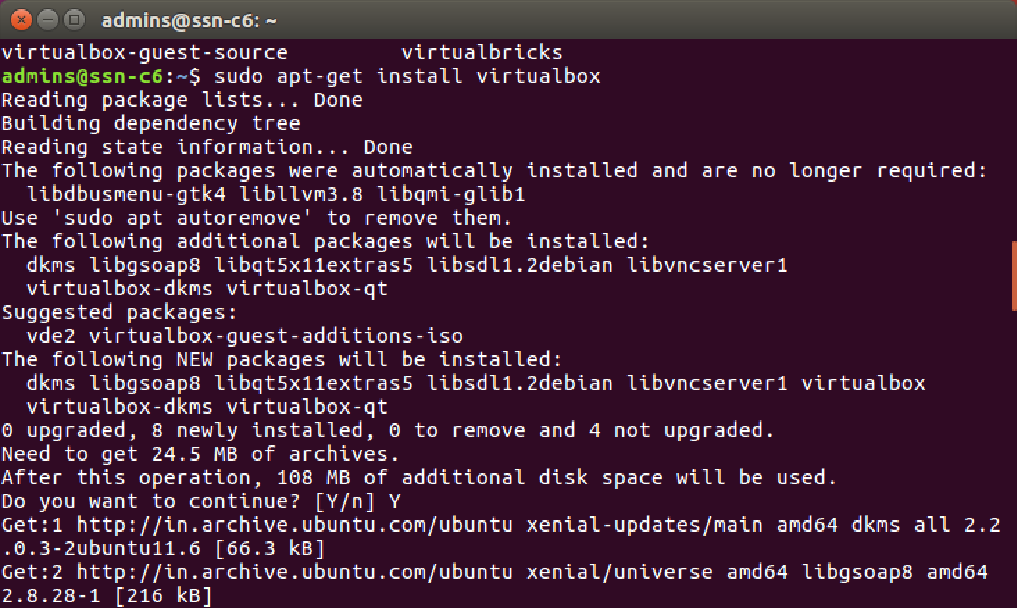
\includegraphics[scale=0.25]{fig1.png}
	\caption{Installing oracle virtualbox in native OS.}
	\label{fig:1}
\end{figure}

\begin{figure}[h]
	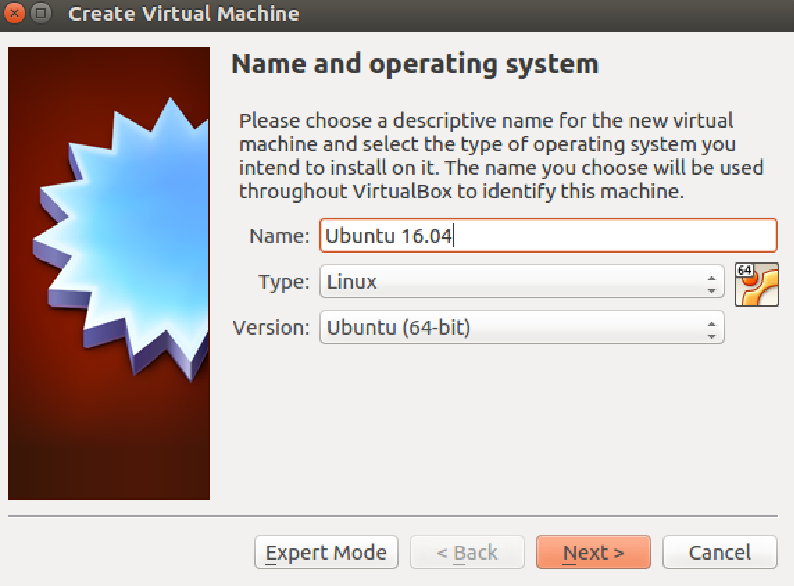
\includegraphics[scale=0.25]{fig2.png}
	\caption{Selecting the operating system flavour as Ubuntu 16.04 in guest OS instance.}
	
	\label{fig:2}
\end{figure}

\begin{figure}[h]
	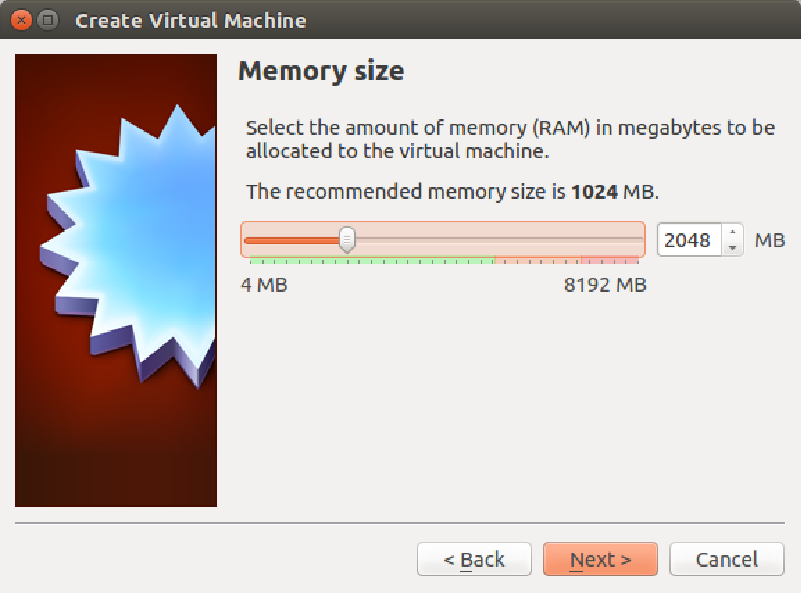
\includegraphics[scale=0.25]{fig3.png}
	\caption{Selecting the required RAM memory space for the VM instance.}
	\label{fig:3}
\end{figure}

\begin{figure}[h]
	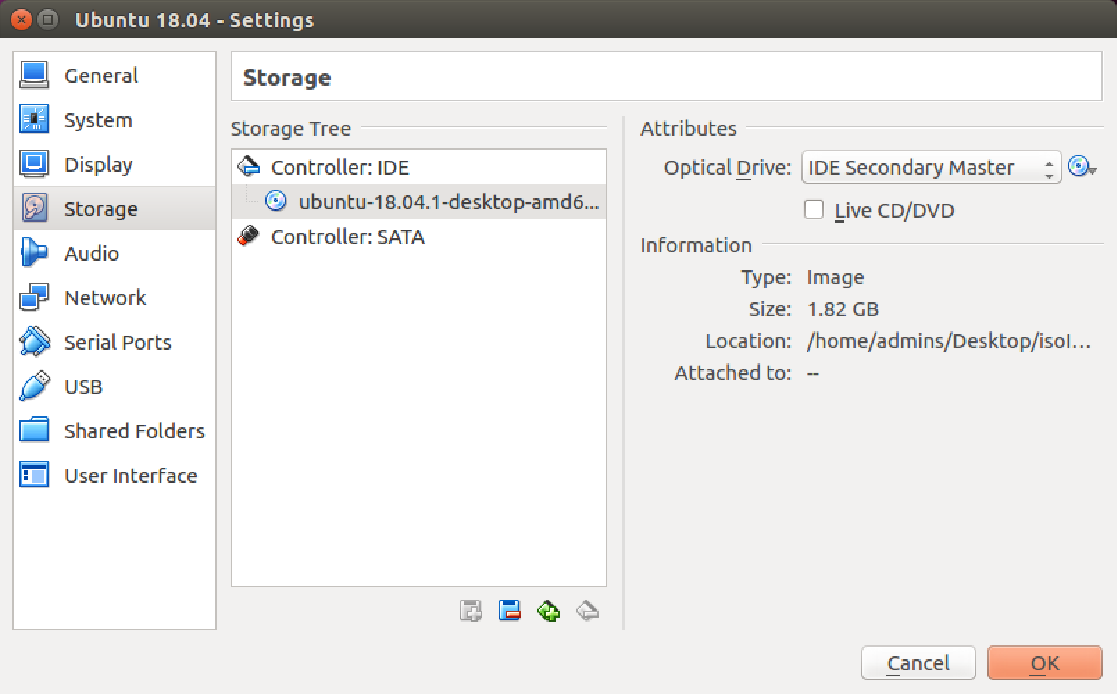
\includegraphics[scale=0.25]{fig4.png}
	\caption{Figure shows the another message box for storing image in \textit{eps} format}
	\label{fig:4}
\end{figure}

\begin{figure}[h]
	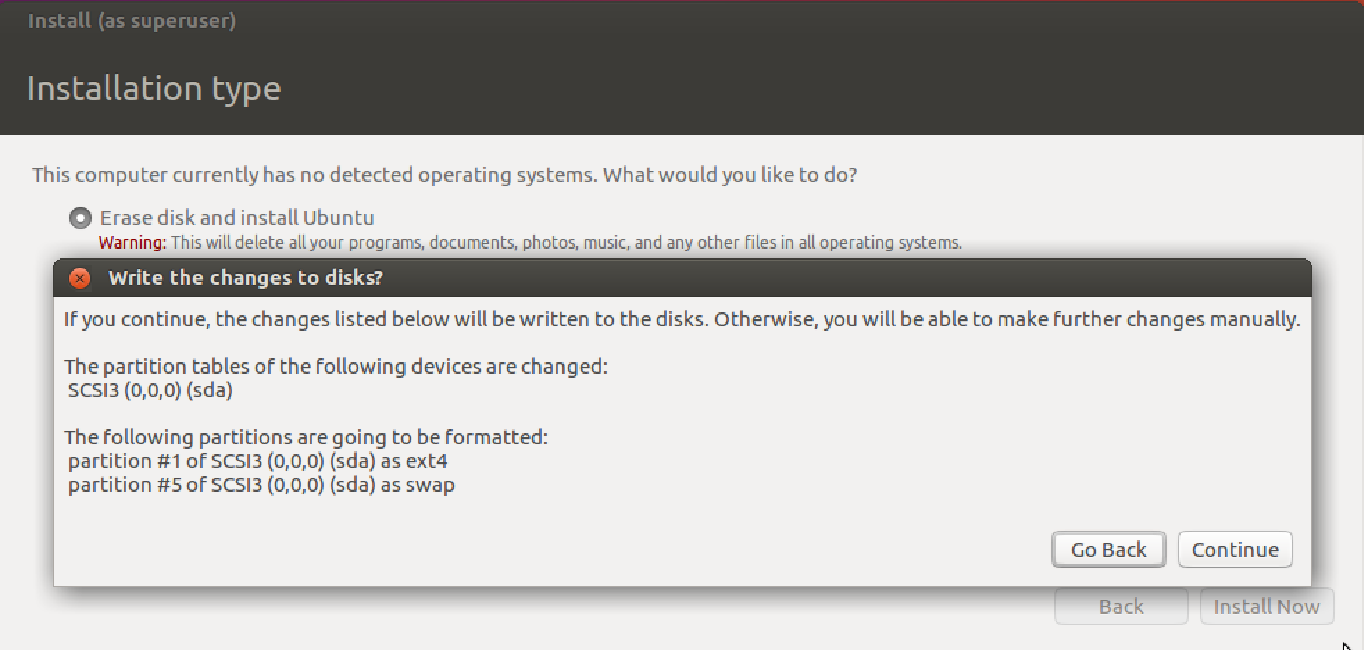
\includegraphics[scale=0.25]{fig5.png}
	\caption{Image Stored in \textit{eps} format}
	\label{fig:5}
\end{figure}

\begin{verbatim}
\begin{figure}[h]
	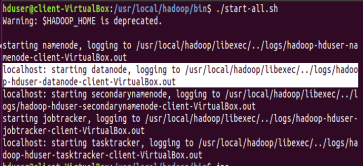
\includegraphics[scale=0.25]{fig1.eps}
	\caption{Image Stored in \textit{eps} format}
	\label{fig:6}
\end{figure}
Here you can file name is changed to \textit{png} to \textit{eps}.
When using \textit{png} image - compile using this option \textit{PdfLatex + View PDF}
When using \textit{eps} image - compile using this option \textit{latex + dvips + ps2pdf + View PDF}
\end{verbatim}

\section{Result}
Thus the C program to convert the equivalent value of rupees entered in digits to words is written and executed successfully. 

\end{document}
